\documentclass[11pt]{beamer}
\newtheorem{proposition}{Proposition}

\usepackage[nosetup]{evan}
\usepackage{derivative}
\usepackage{mathrsfs}
\usepackage{booktabs}
\usepackage{multirow}
\usetheme{Malaysia}

\usepackage{tikz-cd}
\usetikzlibrary{decorations.pathmorphing}

\usepackage{fontspec}
\directlua{luaotfload.add_fallback
  ("evans_fallbacks",
    {
      "NotoColorEmoji:mode=harf;",
      "Source Han Sans TW:style=Regular;",
      "Noto Serif CJK SC:style=Regular;",
    }
  )}
\setmainfont{lmroman10-regular}[
  BoldFont=lmroman10-bold,
  ItalicFont=lmroman10-italic,
  BoldItalicFont=lmroman10-bolditalic,
  SlantedFont=lmromanslant10-regular,
  BoldSlantedFont=lmromanslant10-bold,
  SmallCapsFont=lmromancaps10-regular,
  RawFeature={fallback=evans_fallbacks}
]
\setsansfont{lmsans10-regular}[
  BoldFont=lmsans10-bold,
  ItalicFont=lmsans10-oblique,
  BoldItalicFont=lmsans10-boldoblique,
  RawFeature={fallback=evans_fallbacks}
]

\setbeamercovered{transparent}

\DeclareMathOperator{\BC}{BC}
\DeclareMathOperator{\Int}{Int}
\DeclareMathOperator{\Lie}{Lie}
\DeclareMathOperator{\Mat}{Mat}
\DeclareMathOperator{\Nm}{Nm}
\DeclareMathOperator{\Orb}{Orb}
\DeclareMathOperator{\Sat}{Satake}
\DeclareMathOperator{\Sh}{Sh}
\DeclareMathOperator{\SO}{SO}
\DeclareMathOperator{\Spf}{Spf}
\DeclareMathOperator{\U}{U}
\DeclareMathOperator{\rproj}{proj}

\newcommand{\G}{\mathrm{G}}
\newcommand{\EE}{\mathbb{E}}
\newcommand{\HH}{\mathcal{H}}
\newcommand{\MM}{\mathcal{M}}
\newcommand{\VV}{\mathbb{V}}
\newcommand{\TT}{\mathbb{T}}
\newcommand{\XX}{\mathbb{X}}
\renewcommand{\H}{\mathrm{H}}
\renewcommand{\OO}{O}

\newcommand{\RZ}{\mathcal{N}}
\newcommand{\Sheaf}{\mathcal O}
\newcommand{\ZD}{\mathcal{Z}}
\newcommand{\guv}{{(\gamma, \uu, \vv^\top)}}
\newcommand{\jiao}{\mathop{\otimes}^{\mathbf{L}}} % this is a cute macro name (交)
\newcommand{\oneV}{\mathbf{1}_{\OO_F^n \times (\OO_F^n)^\vee}}
\newcommand{\rs}{_{\text{rs}}}
\newcommand{\uu}{\mathbf{u}}
\newcommand{\vv}{\mathbf{v}}
\newcommand{\ZO}[1]{\mathcal Z^{\dagger}_{\SO(#1)}}

\title[Semi-Lie AFL for full Hecke algebra]{Semi-Lie Arithmetic Fundamental Lemma for full spherical Hecke Algebra}
\institute{Mass Tech}
\author{Evan Chen}
\date{11 December 2024}

\begin{document}

\begin{frame}
  \frametitle{Semi-Lie Arithmetic Fundamental Lemma for full spherical Hecke Algebra}
  \begin{center}
    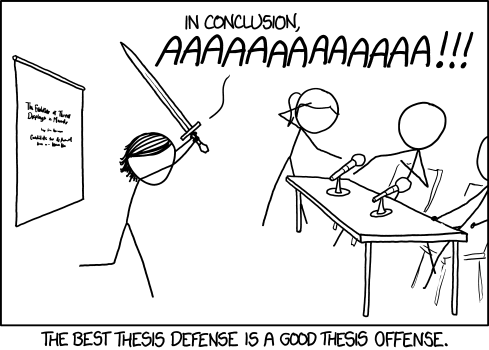
\includegraphics[width=0.8\textwidth]{xkcd.png}
  \end{center}
\end{frame}

\begin{frame}
  \maketitle
\end{frame}

\begin{frame}
  \frametitle{Notation}
  \begin{itemize}
  \ii $E/F$ an unramified quadratic extension of $p$-adic fields, $p > 2$
  \ii $q$ residue characteristic of $F$.
  \ii $\VV_n^+$ split $E/F$-Hermitian space of dimension $n$
  \ii $\VV_n^-$ non-split $E/F$-Hermitian space of dimension $n$
  \ii Symmetric space:
  \[ S_n(F) \coloneqq \left\{ \gamma \in \GL_n(E) \mid \gamma\bar\gamma = 1_n \right\} . \]
  \end{itemize}
  Hecke algebras:
  \begin{itemize}
  \ii $\HH(\U(\VV_n^+)) \coloneqq \QQ[K \backslash \U(\VV_n^+) \slash K]$
  is the Hecke algebra of compactly supported $K$-bi-invariant functions,
  where $K \coloneqq \U(\VV_n^+) \cap \GL_n(\OO_E)$ is hyperspecial maximal compact subgroup.
  \ii $\HH(\GL_n(E)) \coloneqq \QQ[K' \backslash \GL_n(E) \slash K']$, $K' \coloneqq \GL_n(\OO_E)$.
  \ii $\HH(S_n(F)) \coloneqq \mathcal C^\infty_{\text{c}} (S_n(F))^{K'}$,
  is an $\HH(\GL_n(E))$-module.
  \end{itemize}
\end{frame}


\begin{frame}
  \frametitle{Overview}
  \centering
  \begin{tabular}{lp{12em}p{8em}}
    \toprule
    \textbf{Conjecture} & \textbf{Lemma} & \textbf{Generalization} \\
    \midrule
    GGP & Fundamental lemma & Leslie (2023) \\ & (Jacquet-Rallis 2011) \\
    \midrule
    \multirow{2}{*}[-1em]{Arith GGP} & AFL for $\U(n) \times \U(n+1)$ (Zhang 2012) & Li-Rapoport-Zhang (2024) \\ \cline{2-3}
    & $\iff$ AFL for $\U(n) \times \U(n)$ (Liu 2021) & 🤔 \\
    \bottomrule
  \end{tabular}
  \begin{block}{Table of contents for talk}
    \begin{itemize}
    \ii Discuss first, second, third column, each from top to bottom.
    \ii Things in first column and first row will be cursory historical overview,
      not defined or made precise at all.
    \end{itemize}
  \end{block}
\end{frame}

\begin{frame}
  \frametitle{GGP/AGGP extremely rough statements}
  %\begin{itemize}
  %\ii Started with Waldspurger 1985 formula
  %  relating automorphic period to $L(1/2)$.
  %\ii Generalized by Gross-Prasad in 1992 and 1994,
  %\ii Generalized further to Gan-Gross-Prossad conjecture (GGP).
  %\end{itemize}
  %Let $k$ be a number field.
  \begin{exampleblock}{Global GGP conjecture, extremely roughly}
    Let $\H \subset \G$ be ``spherical'' pair of reductive groups,
    $\pi$ a tempered cuspidal automorphic representation of $\G$.
    Then the following are equivalent:
    \begin{enumerate}
      \ii $\mathscr P(\phi) \coloneqq \int_{\H(k) \backslash \H(\mathbb A_k)} \phi(h) \odif h$
      is not identically zero for $\phi \in \pi$.
      \ii $\Hom_{\H(\mathbb A_k)}(\pi, \CC) \neq 0$ and $L(\half, \pi , R) \neq 0$
      for certain $R$.
    \end{enumerate}
  \end{exampleblock}
  \begin{exampleblock}{Arithmetic GGP conjecture, extremely roughly}
    Let $\pi$ be a tempered cuspidal automorphic representation of $\G(\mathbb A_k)$
    appearing in the cohomology $H^\bullet(\Sh(\G))$.
    The following are equivalent:
    \begin{enumerate}
      \ii A certain height pairing
      $\mathscr{P}_{\Sh(\H)} \colon \opname{Ch}^{n-1}(\Sh(\G))_0 \to \CC$
      does not vanish on $\pi_f$-isotypic component.
      \ii $\Hom_{\H(\mathbb{A}_k)}(\pi_f, \CC) \neq 0$
      and $L'(\half, \pi, R) \neq 0$ for certain $R$.
    \end{enumerate}
  \end{exampleblock}
\end{frame}

%\begin{frame}
%  \frametitle{What Arithmetic GGP looks like, extremely roughly}
%  \begin{itemize}
%  \ii Started with Gross-Zagier (1986), relating height of Heegner point on modular curve to $L'(s)$ at $s = 1$
%  \ii Yuan-Zhang-Zhang (2013) proved generalization to Shimura curve over totally real field.
%  \ii Arith.~GGP further generalizes to higher dimensional Shimura variety.
%  \end{itemize}
%  %Beginning from a spherical pair $(\H,\G)$,
%  %upgrade to Shimura data $(\H, X_\H) \to (\G, X_\G)$.
%  \begin{exampleblock}{Arithmetic GGP conjecture, extremely roughly}
%    Let $\pi$ be a tempered cuspidal automorphic representation of $\G(\mathbb A_k)$
%    appearing in the cohomology $H^\bullet(\Sh(\G))$.
%    The following are equivalent:
%    \begin{enumerate}
%      \ii A certain height pairing
%      \[ \mathscr{P}_{\Sh(\H)} \colon \opname{Ch}^{n-1}(\Sh(\G))_0 \to \CC \]
%      does not vanish on $\pi_f$-isotypic component.
%      \ii $\Hom_{\H(\mathbb{A}_k)}(\pi_f, \CC) \neq 0$
%      and $L'(\half, \pi, R) \neq 0$ for certain $R$.
%    \end{enumerate}
%  \end{exampleblock}
%\end{frame}

\begin{frame}
  \frametitle{Jacquet-Rallis fundamental lemma}
  \begin{itemize}
  \ii $(\VV_n^+)^\flat$ codimension one subspace in $\VV_n^+$.
  \ii $G'^\flat \coloneqq \GL_{n-1}(E)$, $G' \coloneqq \GL_n(E)$,
    $G^\flat \coloneqq \U((\VV_n^+)^\flat)(F)$, $G \coloneqq \U(\VV_n^+)(F)$.
  \ii $K'^\flat$, $K'$, $K^\flat$, $K$ maximal hyperspecial compact subgroups.
  \end{itemize}
  \begin{block}{Fundamental lemma, roughly}
    For certain ``matching''
    $\gamma \in G'^\flat \times G'$ and $g \in G^\flat \times G$
    we get
   \[ \Orb(\gamma, \mathbf{1}_{K'^\flat \times K'}) = \pm \Orb(g, \mathbf{1}_{K^\flat \times K}) \]
  \end{block}
  %Now proved completely; a local proof was given by Beuzart-Plessis (2021)
  %while a global proof was given for large characteristic by W.\ Zhang (2021).
\end{frame}
\begin{frame}
  \frametitle{Arithmetic fundamental lemma}
  Analogous statement to Jacquet-Rallis fundamental lemma.
  For simplicity, stating the inhomogeneous version (the full version is more general).
  \begin{definition}
  For $\gamma \in S_n(F)$, $\phi \in \HH(S_n(F))$, and $s \in \CC$:
  \[ \Orb(\gamma, \phi, s) \coloneqq
    \int_{h \in \GL_{n-1}(F)} \phi(h\inv \gamma h) (-1)^{v(\det h)}
    \left\lvert \det(h) \right\rvert_F^{-s} \odif h. \]
  \end{definition}
  \begin{theorem}
  [Inhomogeneous AFL]
  For matching regular semisimple elements
  $g \in \U(\VV_n^-)\rs \longleftrightarrow \gamma \in S_n(F)\rs$:
  \[
    \Int\left( (1,g), \mathbf{1}_{K'^\flat} \otimes \mathbf{1}_{K'} \right) \log q
    = \pm \left. \pdv{}{s} \right\rvert_{s=0} \Orb(\gamma, \mathbf{1}_K, s).
  \]
  \end{theorem}
\end{frame}

%\begin{frame}
%  \frametitle{Regular semisimple definition}
%  \begin{itemize}
%    % \ii The matrix $A$ is $(n-1) \times (n-1)$.
%    \ii Write $\GL_n(E)\rs$ to denote semisimple elements.
%    \ii Equivalent to requiring that, under the action of conjugation by $\GL_{n-1}(E)$:
%    the matrix has trivial stabilizer; and
%    the $\GL_{n-1}(\ol E)$-orbit is a Zariski-closed subset of $\GL_n(\ol E)$.
%  \end{itemize}
%  Regular semisimple elements are acted on by conjugation under $\GL_{n-1}(E)$
%  (viewed as a subset of $\GL_n(E)$ by $g \mapsto \begin{pmatrix} g & 0 \\ 0 & 1 \end{pmatrix}$.)
%\end{frame}

\begin{frame}
  \frametitle{Matching definition}
  %Orbits are classified by the following invariants:
  %\begin{itemize}
  %  \ii The matrices $A_1$ and $A_2$ have the same characteristic polynomial;
  %  \ii We have $\vv_1^\top A_1^i \uu_1 = \vv_2^\top A_2^i \uu_2$
  %  for every $i = 0, 1, \dots, n-2$; and
  %  \ii We have $d_1 = d_2$.
  %\end{itemize}
  \begin{definition}
  $\begin{pmatrix} A & \uu \\ \vv^\top & d \end{pmatrix} \in \GL_n(E)$
  is \textbf{regular semisimple} if
  \[ \Delta \coloneqq \det \left( \left( \vv^\top A^{i+j-2} \uu \right)_{i,j=1}^{n-1} \right) \neq 0 \]
  We say $\gamma \in S_n(F)\rs$ \textbf{matches} the element $g \in \U(\VV_n^\pm)\rs$
  if $g$ is conjugate to $\gamma$ by an element of $\GL_{n-1}(E)$; write
  $g \in \U(\VV_n^\pm)\rs \longleftrightarrow \gamma \in S_n(F)\rs$.
  \end{definition}
  \begin{block}{Matching criteria}
    \[ [S_n(F)]\rs \xrightarrow{\sim} [\U(\VV_n^+)]\rs \amalg [\U(\VV_n^-)]\rs. \]
    Matches in $\U(\VV_n^+)$ if $v(\Delta)$ is even,
    and $\U(\VV_n^-)$ otherwise.
  \end{block}
\end{frame}

%\begin{frame}
%  \frametitle{Weighted orbital integral definition}
%  For comparison, the unweighted orbital for $f \in \HH(\U(\VV_n^+))$ is:
%  \[ \Orb^{\U(\VV_n^+)}(g, f) \coloneqq \int_{\U(\VV_n^+)} f(x^{-1}gx) \odif x \]
%  \begin{theorem}
%    [Relative fundamental lemma; Leslie 2023]
%    Suppose $\phi$ and $f$ are related by \emph{base change}, and $\gamma \longleftrightarrow g$, then:
%    \[
%      \pm \Orb(\phi, \gamma, 0)
%      = \begin{cases}
%        0 & v(\Delta) \text{ odd (AFL case)} \\
%        \Orb^{\U(\VV_n^+)}(g, f) & v(\Delta) \text{ even}.
%      \end{cases}
%    \]
%  \end{theorem}
%\end{frame}

\begin{frame}
  \frametitle{Rapoport-Zink space}
  \begin{itemize}
    \ii Let $\breve F$ denote the completion of a maximal unramified extension of $F$,
    and let $\FF$ denote the residue field of $\OO_{\breve F}$.
    \ii Suppose $S$ is a $\Spf \OO_{\breve F}$-scheme.
  \end{itemize}
  \begin{definition}
  Consider triples $(X, \iota, \lambda)$ where:
  \begin{itemize}
    \ii $X$ is a formal $\varpi$-divisible $n$-dimensional $\OO_F$-module over $S$
    whose relative height is $2n$.

    \ii $\iota \colon \OO_E \to \End(X)$ is an action of $\OO_E$
    such that the induced action of $\OO_F$ on $\Lie X$
    is via the structure morphism $\OO_F \to \Sheaf_S$,
    satisfying the Kottwitz condition of signature $(n-1,1)$,

    \ii $\lambda \colon X \to X^\vee$ is a principal $\OO_F$-relative polarization
    whose Rosati involution induces $a \mapsto \bar a$ on $\OO_F$.
   \end{itemize}
  \end{definition}
\end{frame}

\begin{frame}
  \frametitle{Rapoport-Zink space, continued}
  Choose a \emph{supersingular} triple $(\XX_n, \iota_{\XX_n}, \lambda_{\XX_n})$
  called the \emph{framing object}.
  \begin{definition}
    For each $n \ge 1$, we let $\RZ_n$ denote the
    functor over $\Spf \OO_{\breve F}$ defined as follows.
    Let $S$ be an $\Spf \OO_{\breve F}$ scheme,
    $\ol S \coloneqq S \times_{\Spf \OO_{\breve F}} \Spec \FF$.
    We let $\RZ_n(S)$ be the set of isomorphism classes of quadruples
    $(X, \iota, \lambda, \rho)$
    where $(X, \iota, \lambda)$ is one of the triples as we described, and
    \[ \rho \colon X \times_S \ol S \to \XX_n \times_{\Spec \FF} \ol S \]
    is a \emph{framing}, meaning it is a height zero $\OO_F$-linear quasi-isogeny
    and satisfies $\rho^\ast((\lambda_{\XX_n})_{\ol S}) = \lambda_{\ol S}$.
  \end{definition}
  Then $\RZ_n$ is formally smooth over $\OO_{\breve F}$ of relative dimension $n-1$
  and is acted on by $\U(\VV_n^-)$.
\end{frame}
\begin{frame}
  \frametitle{Intersection number}
  \begin{itemize}
    \ii $\RZ_{m,n} \coloneqq \RZ_m \times \RZ_n$.
    \ii Let $\Delta \colon \RZ_{n-1} \to \RZ_{n-1,n}$
    be the graph morphism of $\delta \colon \RZ_{n-1} \to \RZ_n$,
    with image $\Delta_{\RZ{n-1}}$.
    \ii Realize $\VV_n^- = \Hom_{\OO_E}^\circ(\EE, \XX_n)$.
  \end{itemize}

  \begin{definition}
    \begin{align*}
      \Int((1,g), \mathbf{1}_{K'^\flat} \otimes \mathbf{1}_{K'})
      &\coloneqq \left( \Delta_{\RZ_{n-1}}, (1,g) \cdot \Delta_{\RZ_{n-1}} \right)_{\RZ_{n-1,n}} \\
      &\coloneqq \chi_{\RZ_{n-1,n}}
      \left( \Sheaf_{\Delta_{\RZ_{n-1}}} \jiao_{\Sheaf_{\RZ_{n-1,n}}} \Sheaf_{(1,g) \cdot \Delta_{\RZ_{n-1}}} \right) .
    \end{align*}
    ($\jiao$ is derived tensor product, $\chi$ is Euler-Poincare characteristic)
  \end{definition}

\end{frame}


\begin{frame}
  \frametitle{Semi-Lie version of AFL by Yifeng Liu (2021)}
  \begin{definition}
  For $\guv \in S_n(F) \times F^n \times (F^n)^\vee$,
  $\phi \in \HH(S_n(F))$, and $s \in \CC$,
  \begin{align*}
    & \Orb((\gamma, \uu, \vv^\top), \phi \otimes \oneV, s) \\
    &\coloneqq \int_{h \in \GL_n(F)} \phi(h\inv \gamma h) \oneV(h \uu, \vv^\top h^{-1})
      (-1)^{v(\det h)} \left\lvert \det(h) \right\rvert_F^{-s} \odif h.
  \end{align*}
  \end{definition}

  \begin{theorem}
    [AFL, semi-Lie version]
    If $(g, u) \in (\U(\VV_n^-) \times \VV_n^-)\rs \longleftrightarrow
      (\gamma, \uu, \vv^\top) \in (S_n(F) \times F^n \times (F^n)^\vee)\rs$:
    \[
      \Int\left( (g,u), \mathbf{1}_{K'} \right) \log q
      = \pm \left. \pdv{}{s} \right\rvert_{s=0}
      \Orb(\guv, \mathbf{1}_K \otimes \oneV, s).
    \]
  \end{theorem}
  Equivalent to Zhang's AFL; induction uses both!
\end{frame}

\begin{frame}
  \frametitle{Matching (analogous)}
  Matching is defined in the same way via
  $(g,u) \mapsto \begin{pmatrix} g & u \\ u^\ast & d \end{pmatrix} \in \GL_{n+1}(E)$
  and $\guv \mapsto \begin{bmatrix} \gamma & \uu \\ \vv^\top & d \end{bmatrix} \in \GL_{n+1}(E)$.

  \begin{block}{Matching criteria in semi-Lie case}
  \[ [S_n(F) \times F^n \times (F^n)^\vee]\rs \xrightarrow{\sim} [\U(\VV_n^+) \times \VV_n^+]\rs \amalg [\U(\VV_n^-) \times \VV_n^-]\rs. \]
  To see which one, define
  \[ \Delta \coloneqq \det \left( \left( \vv^\top \gamma^{i+j-2} \uu \right)_{i,j=1}^n \right) \neq 0. \]
  We get $\VV_n^+$ if $v(\Delta)$ is even
  and $\VV_n^-$ if $v(\Delta)$ is odd.
  \end{block}
\end{frame}

%\begin{frame}
%  \frametitle{Weighted orbital integral}
%  Unweighted version, where $f \in \HH(\U(\VV_n^+))$,
%  and $\Lambda_n$ is a self-dual lattice:
%  \[
%    \Orb^{\U(\VV_n^+) \times \VV_n^+}\left( (g,u), f \otimes \mathbf{1}_{\Lambda_n} \right)
%    \coloneqq \int_{\U(\VV_n^+)} f(x\inv g x) \mathbf{1}_{\Lambda_n}(x^{-1} u) \odif x.
%  \]
%  \begin{exampleblock}{Conjecture}
%    If $\phi$ and $f$ are related by \emph{base change},
%    $\guv \longleftrightarrow (g,u)$, then:
%    \[ \pm \Orb(\dots)
%      =
%      \begin{cases}
%        0 & v(\Delta) \text{ odd (AFL case)} \\
%        \Orb^{\U(\VV_n^+) \times \VV_n^+}\left( \dots \right)
%        & v(\Delta) \text{ even}.
%      \end{cases}
%    \]
%  \end{exampleblock}
%\end{frame}

\begin{frame}
  \frametitle{Intersection number (briefly)}
  \begin{definition}
    Let $(\EE, \iota_\EE, \lambda_\EE)$ be the unique triple over $\FF$
    which has signature $(1,0)$.
    Then the formal $\OO_F$-module has a unique lifting called its \emph{canonical lifting},
    denoted $(\mathcal{E}, \iota_{\mathcal{E}}, \lambda_{\mathcal E})$.
    The \alert{Kudla-Rapoport divisor $\ZD(u)$}
    is the locus where the quasi-homomorphism $\EE \to \XX_n$ lifts to a homomorphism
    from $\mathcal{E}$ to the universal object over $\RZ_n$.
  \end{definition}
  Let $\Delta_{\ZD(u)}$ be the image of $\ZD(u) \to \RZ_n \to \RZ_{n,n}$;
  let $\Gamma_g \subseteq \RZ_{n,n}$ be the graph of the automorphism of $\RZ_n$ induced by $g$.
  \begin{definition}
    \[
      \Int((g,u), \mathbf{1}_{K'})
      \coloneqq \left( \Delta_{\ZD(u)}, \Gamma_g \right)_{\RZ_{n,n}}
      \coloneqq \chi_{\RZ_{n,n}}
      \left( \Sheaf_{\Delta_{\ZD(u)}} \jiao_{\Sheaf_{\RZ_{n,n}}} \Sheaf_{\Gamma_g}  \right).
    \]
  \end{definition}
\end{frame}

\begin{frame}[fragile]
  \frametitle{Base change}
  Denote by $\rproj \colon \GL_n(E) \surjto S_n(F)$ the map $\rproj(g) \coloneqq g \bar{g}\inv$.
  \begin{align*}
    \rproj^{\eta^{n-1}}_\ast \colon \HH(\GL_n(E)) &\to \HH(S_n(F)) \\
    \rproj^{\eta^{n-1}}_\ast(f')\left( g\bar{g}\inv \right) &= \int_{\GL_n(F)} f'(gh) \eta^{n-1}(gh) \odif h
  \end{align*}
  And let $\eta(g) = (-1)^{v(\det g)}$ be the nontrivial quadratic character for $E/F$.
  \begin{center}
  \begin{tikzcd}
    & \HH(\GL_n(E)) \ar[ld, "\rproj_\ast^{\eta^{n-1}}"'] \ar[r, "\sim"', "\Sat"] \ar[d, "\BC"]
      & \QQ[X_1^\pm, \dots, X_n^\pm]^{\opname{Sym}(n)} \ar[d, "\BC"] \\
    \HH(S_n(F)) \ar[r, "\sim", "\BC_{S_n}^{\eta^{n-1}}"'] & \HH(\U(\VV_n^+)) \ar[r, "\sim"', "\Sat"]
      & \QQ[Y_1^\pm, \dots, Y_m^\pm]^{W_m} \\
  \end{tikzcd}
  \end{center}
  \begin{theorem}
    [Leslie 2023]
    $\BC$ factors through $\rproj_\ast^{\eta^{n-1}}$
    and gives an isomorphism $\BC_{S_n}^{\eta^{n-1}}$.
  \end{theorem}
\end{frame}


\begin{frame}
  \frametitle{Leslie's generalization of Jacquet-Rallis fundamental lemma to the full spherical Hecke algebra}
  As before $G'^\flat \coloneqq \GL_{n-1}(E)$, $G' \coloneqq \GL_n(E)$,
  $G^\flat \coloneqq \U((\VV_n^+)^\flat)(F)$, $G \coloneqq \U(\VV_n^+)(F)$.

  \begin{theorem}[Leslie 2023]
    Suppose \alert{$\varphi'$ and $\varphi$ are related by base change}; then still
    for certain ``matching'' $\gamma \in G'^\flat \times G'$ and $g \in G^\flat \times G$:
    \[ \Orb(\gamma, \alert{\varphi'}) = \pm \Orb(g, \alert{\varphi}). \]
  \end{theorem}

  The original Jacquet-Rallis fundamental lemma is the special case
  \begin{align*}
    \varphi' = \mathbf{1}_{K'^\flat \times K'} &\in \HH(\GL_{n-1}(E)) \otimes \HH(\GL_n(E)) \\
    \varphi = \mathbf{1}_{K^\flat \times K} &\in \HH(\U((\VV_n^+)^\flat)) \otimes \HH(\U(\VV_n^+)).
  \end{align*}
\end{frame}

\begin{frame}
  \frametitle{AFL conjectured for the full spherical Hecke algebra}
  \begin{exampleblock}{Conjecture (Li-Rapoport-Zhang 2024)}
    Let \alert{$f \in \HH(\U(\VV_n^+))$} and \alert{$\phi \in \HH(S_n(F))$}
    be \alert{related by base change}.
    Then for matching $g \in \U(\VV_n^-)\rs \longleftrightarrow \gamma \in S_n(F)\rs$:
    \[ \Int\left( (1,g), \mathbf{1}_{K^\flat} \otimes \alert{f} \right) \log q
    = \pm \left. \pdv{}{s} \right\rvert_{s=0} \Orb(\gamma, \alert{\phi}, s). \]
  \end{exampleblock}
  AFL is special case $f = \mathbf{1}_{K}$ and $\phi = \mathbf{1}_{K'}$.
  Verified for $n = 2$. \\
  (For $n=3$, I brute-force computed RHS but not LHS.)
  \begin{block}{Updated intersection number
    (with new Hecke operator $\TT_{\mathbf{1}_{K^\flat} \otimes f}$)}
    \[
      \Int((1,g), \mathbf{1}_{K^\flat} \otimes f)
      \coloneqq \chi_{\RZ_{n-1,n}} \left(
        \Sheaf_{\alert{\TT_{\mathbf{1}_{K^\flat} \otimes f}} (\Delta_{\RZ_{n-1}})}
        \jiao_{\Sheaf_{\RZ_{n-1,n}}} \Sheaf_{(1,g) \cdot \Delta_{\RZ_{n-1}}} \right).
    \]
  \end{block}
\end{frame}

\begin{frame}
  \frametitle{Semi-Lie AFL conjectured for full spherical Hecke algebra}
  \begin{exampleblock}{Conjecture (C., October 2024)}
    Let \alert{$f \in \HH(\U(\VV_n^+))$} and \alert{$\phi \in \HH(S_n(F))$}
    be \alert{related by base change}, and
    \[ (g, u) \in (\U(\VV_n^-) \times \VV_n^-)\rs \longleftrightarrow
    (\gamma, \uu, \vv^\top) \in (S_n(F) \times \OO_F^n \times (\OO_F^n)^\vee)\rs. \]
    Then
    \[
      \Int\left( (g,u), \alert{f} \right) \log q
      = \pm \left. \pdv{}{s} \right\rvert_{s=0}
      \Orb(\guv, \alert{\phi} \otimes \oneV, s).
    \]
  \end{exampleblock}
  \begin{block}{Updated definition of intersection number}
    \[
      \Int((g,u), f)
      \coloneqq \chi_{\RZ_{n,n}} \left(
      \Sheaf_{\alert{\TT_{\mathbf{1}_K \otimes f}}(\Delta_{\ZD(u)})}
      \jiao_{\Sheaf_{\RZ_{n,n}}} \Sheaf_{\Gamma_g} \right).
    \]
  \end{block}
\end{frame}
\begin{frame}
  \begin{exampleblock}{Main theorem}
    Semi-Lie AFL conjecture holds when $n = 2$.
  \end{exampleblock}
  \begin{block}{Strategy of proof for $n = 2$}
    \begin{itemize}
      \ii For $n = 2$, on the orbital side use indicator functions of
      \[ K'_{S, \le r} \coloneqq S_2(F) \cap \varpi^{-r} \GL_2(\OO_E) \]
      as a basis of $\HH(S_2(F))$, for $r \ge 0$.
      \ii Straightforward to get base change to $\HH(\U(\VV_2^+))$ which has a similar basis
      \[ \mathbf{1}_{K, r} \coloneqq
        \mathbf{1}_{\varpi^{-r} \Mat_2(\OO_E) \cap \U(\VV_2^+)} \in \HH(\U(\VV_2^+)). \]
      \ii On the geometric side, work instead with a Lubin-Tate space $\mathcal{M}_2$
      by pulling back with Serre tensor construction.
    \end{itemize}
  \end{block}
\end{frame}

\begin{frame}
  \frametitle{Example $\Orb(\guv, \mathbf{1}_{K'_{S, \le r}} \otimes \oneV)$ when $n=2$}
  \[ \guv = \left( \begin{pmatrix} a & b \\ c & d \end{pmatrix},
      \begin{pmatrix} 0 \\ 1 \end{pmatrix},
      \begin{pmatrix} 0 & e \end{pmatrix} \right) \]
  For $r=2$, $v(d-a)=1$, $v(b)=3$, $v(c)=0$, $v(e)=5$:
  \begin{align*}
    \Orb(\dots) &= -q^{-5s} &&+ (3q^3+q^2+q+1) q^{4s} \\
    &+ q^{-4s} &&- (2q^3+q^2+q+1) q^{5s} \\
    &- (q+1) q^{-3s} &&+ (q^3+q^2+q+1) q^{6s} \\
    &+ (q+1) q^{-2s} &&- (q^2+q+1) q^{7s} \\
    &- (q^2+q+1) q^{-s} &&+ (q^2+q+1) q^{8s} \\
    &+ (q^2+q+1) &&- (q+1) q^{9s}\\
    &- (q^3+q^2+q+1) q^{s} &&+ (q+1)q^{10s} \\
    &+ (2q^3+q^2+q+1) q^{2s} &&- q^{11s} \\
    &- (3q^3+q^2+q+1) q^{3s} &&+ q^{12s}. \\
  \end{align*}
\end{frame}

\begin{frame}[fragile]
  \begin{definition}[Lubin-Tate space $\MM_2$]
    We let $\MM_2$ denote the functor over $\Spf \OO_{\breve F}$ similarly
    by taking the set of isomorphism classes of quadruples
    $(Y, \iota, \lambda, \rho)$ where $(Y, \iota, \lambda)$ is as before and
    $\rho \colon Y \times_S \ol S \to \EE \times_{\Spec \FF} \ol S$
    is a framing.
  \end{definition}
  \begin{definition}[The divisor $\ZO4(u)$ on $\MM_2 \times \MM_2$]
    Define divisor $\ZO4(u)$ to be the pairs $(Y, Y') \in \MM_2 \times \MM_2$
    such that there exists $\varphi \colon Y \to Y'$ for which
    the given $u \colon \EE \to \EE$ lifts to
    \begin{center}
    \begin{tikzcd}
      Y \times_S \ol S \ar[rr, "\varphi \times_S \ol S"] \ar[d, "\rho"] && Y' \times_S \ol S\ar[d, "\rho'"] \\
      \EE \times_{\Spec \FF} \ol S \ar[rr, "u \times_{\Spec \FF} \ol S"] && \EE \times_{\Spec \FF} \ol S.
    \end{tikzcd}
    \end{center}
  \end{definition}
\end{frame}

\begin{frame}
  \frametitle{Gross-Keating}
  \begin{itemize}
    \ii Since $\RZ_2 \simeq \MM_2$ work on $\MM_2$ instead.
    \ii The Hecke correspondence gives $\TT_{\mathbf{1}_K \otimes f}(\Delta_{\RZ_2}) \simeq \ZO4(\varpi^r)$.
    \ii $\U(\VV_2^-)$ can basically be identified with $\SO(3)$, up to certain tori.
    \ii Use Gross-Keating triple product formula on $\MM_2$.
  \end{itemize}
  \begin{theorem}
    [Gross-Keating triple product formula]
    \bgroup
    \small
    $n_1 = \min\left( v((x,x) ), v( (x,y) ), v( (y,y) ) \right)$;
    $n_1 + n_2 = v\left( (x,x) (y,y) - (x,y)^2 \right)$
    \egroup
    \begin{align*}
      &\left< \ZO4(1), \; \ZO4(x), \; \ZO4(y) \right>_{\MM_2 \times \MM_2} \\
      &=
      \begin{cases}
        \sum_{j=0}^{\frac{n_1-1}{2}} (n_1+n_2-4j) q^j & n_1 \text{ odd} \\
        \frac{n_2-n_1+1}{2} q^{n_1/2} + \sum_{j=0}^{n_1/2-1} (n_1+n_2-4j) q^j & n_1 \text{ even}.
      \end{cases}
    \end{align*}
  \end{theorem}
\end{frame}

\begin{frame}
  \frametitle{An example of part of the intersection number}
  \[ \ZD(u)^\circ \coloneqq \ZD(u) - \ZD\left( \frac{u}{\varpi} \right). \]
  Let $r \ge 1$ and $v(\Nm u) > 0$ for $u \in \VV_2^-$, and let
  \[ g = \lambda^{-1}
    \begin{pmatrix} \alpha & \bar\beta \varpi \\ \beta & \bar\alpha \end{pmatrix}
    \in \U(\VV_2^-) \]
  where $v(\lambda) = 0$.
  With $\mathbb{T}_{\mathbf{1}_K \otimes \mathbf{1}_{K, r}}$ the Hecke operator on $\MM_2$,
  \[ \Big\langle \mathbb{T}_{\mathbf{1}_K \otimes \mathbf{1}_{K, r}}
    \Delta_{\ZD(u)^\circ}, \Gamma_g \Big\rangle_{\RZ_{2,2}}
    =
    \begin{cases}
      (C+1) q^{N} + (C+2) q^{N-1} \\
      2q^N \\
      q^N + q^{N-1}
    \end{cases}
  \]
  where $N = \min(v(\Nm u), v(\beta) + r, v(\alpha-\bar\alpha) + r)$
  and $C = v(\beta) - v(\alpha - \bar\alpha)$.
\end{frame}

\begin{frame}
  \frametitle{Large kernel}
  \begin{itemize}
  \ii Li-Rapoport-Zhang noticed the orbital derivative had a large kernel in group AFL.
  \ii For $n=2$, the set of $\phi \in \HH(S_2(F))$ for which
    \[ \left. \pdv{}{s} \right\rvert_{s=0} \Orb \left(\gamma, \phi, s \right) = 0 \]
    holds identically for all applicable $\gamma \in S_2(F)\rs$
    in fact has codimension $2$.
  %\ii Conjectured the kernel is large for all $n \ge 2$.
  \end{itemize}
  We hope for something similar for semi-Lie, but the situation is different!
\end{frame}
\begin{frame}
  \frametitle{Semi-Lie large image conjecture}
  \[ \partial\Orb \colon \phi \mapsto \left( \guv \mapsto \partial \Orb \left(\guv, \phi \right) \right) \]
  \begin{block}{Conjecture (C.)}
    $\partial\Orb \colon \HH(S_n(F)) \to C^\infty\left( (S_n(F) \times V'_n(F))^- \right)$
    is injective.
  \end{block}
  \begin{theorem}
    [C.]
    True for $n=2$. In fact for $n=2$:
    \begin{enumerate}
    \item[(a)] Still injective even if one only considers $(\gamma, \uu, \varpi^\ZZ \vv^\top)$.

    \item[(b)] But if one requires $v(\uu\vv^\top) \le N$
    then the kernel has codimension at most $N + 2$.
    \end{enumerate}
  \end{theorem}
\end{frame}

\begin{frame}
  \frametitle{The end}
  Slides and thesis draft at
  \href{https://github.com/vEnhance/evans-phd-notebook}{\ttfamily\color{blue} github.com/vEnhance/evans-phd-notebook}
  \begin{center}
    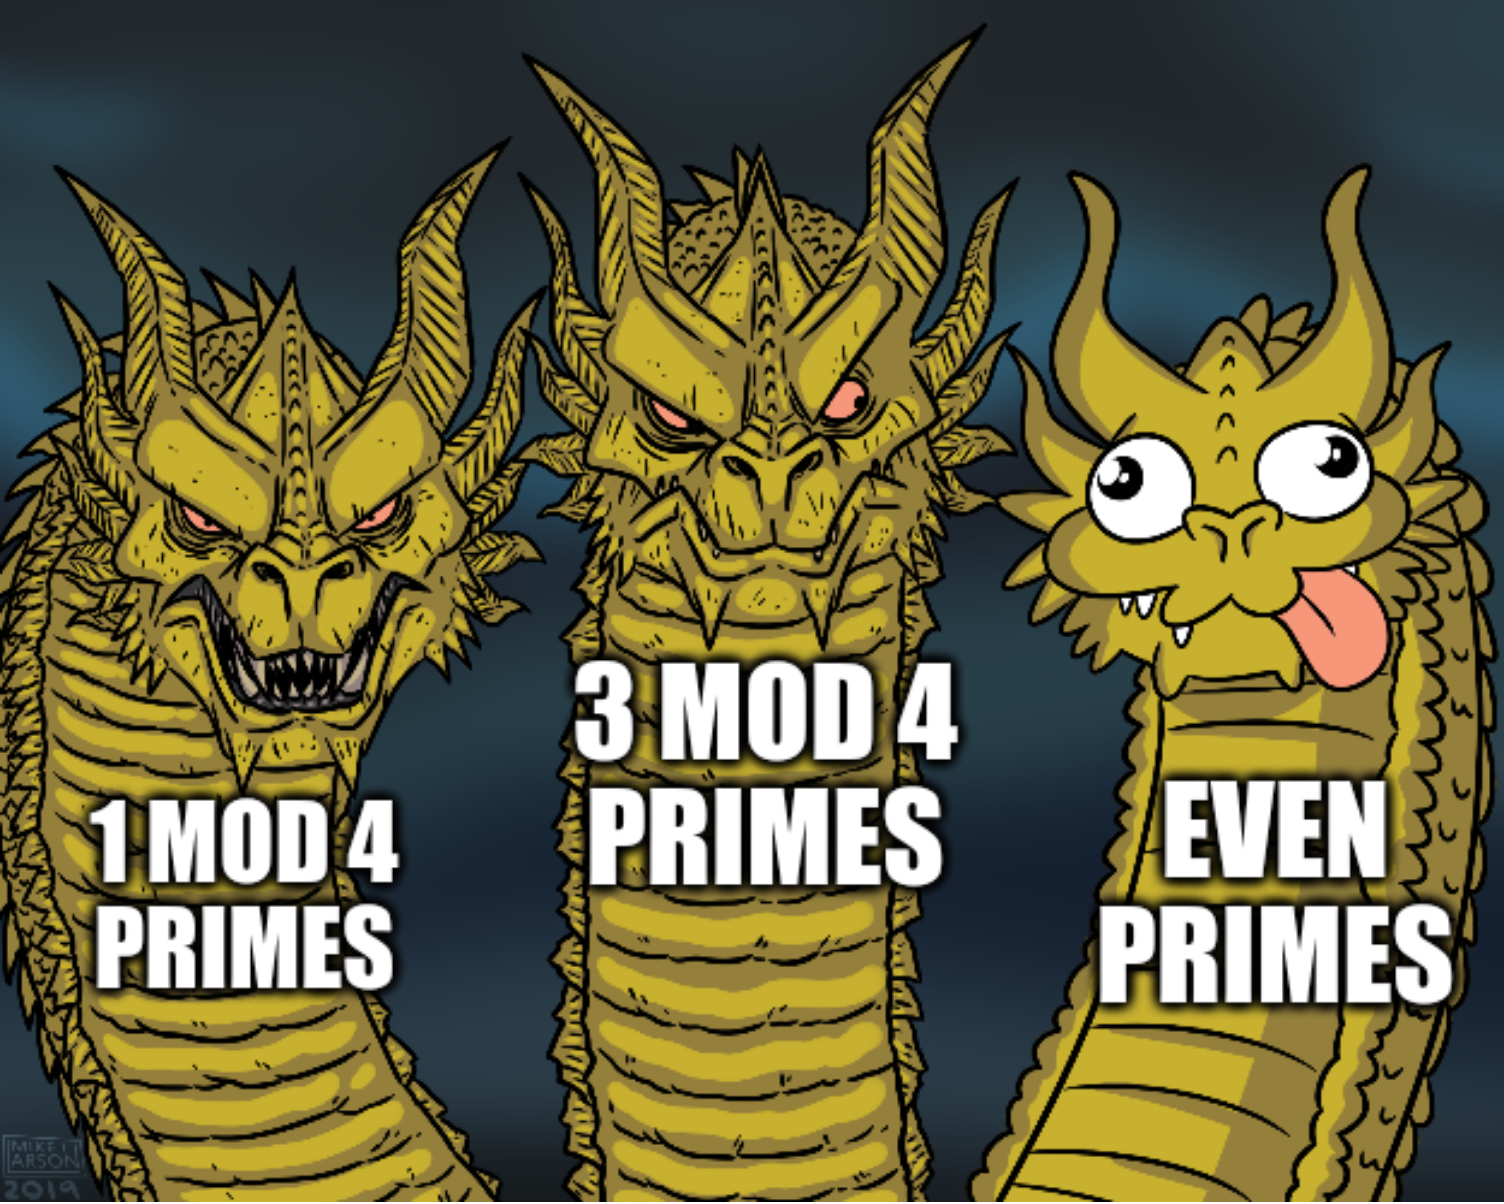
\includegraphics[width=0.7\textwidth]{primes.png}
  \end{center}
\end{frame}

\end{document}
